\title{ Password Lab7 }
\author{Joe}
\date{\today}

\documentclass[12pt]{article}

\usepackage{float}
\usepackage{tikz}
\usetikzlibrary{shapes,arrows}

\usepackage{listings}
\definecolor{mygreen}{rgb}{0,0.6,0}
\definecolor{mygray}{rgb}{0.5,0.5,0.5}
\definecolor{mymauve}{rgb}{0.58,0,0.82}

\usepackage{graphicx}
\graphicspath{ {Images} }

\lstset{numbers=left,commentstyle=\color{mygreen},keywordstyle=\color{blue}}


\begin{document}
\maketitle
\pagebreak

% Source Code
% ===========

\section{Source Code}

Source code for \textsf{app.py}
\lstinputlisting[language=python,breaklines=true]{app.py}

% Menu list imported from instructions
% \lstinputlisting[language=python,breaklines=true]{../menu.yaml}

\newpage

\begin{figure}[H]
  \centering
  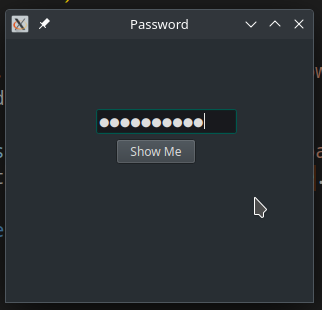
\includegraphics[height=7cm]{ex1.png}
\end{figure}

\begin{figure}[H]
  \centering
  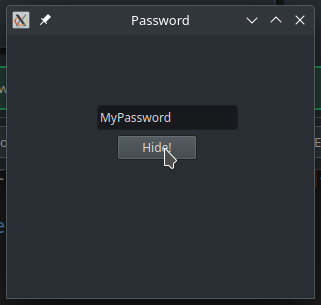
\includegraphics[height=7cm]{ex2.png}
\end{figure}

\begin{figure}[H]
  \centering
  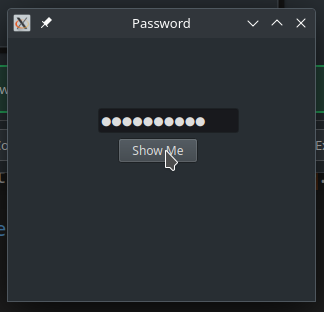
\includegraphics[height=7cm]{ex3.png}
\end{figure}

\newpage

Autogenerated using scripts by Joe and \LaTeX.

Please find the full source code and binaries included.

\end{document}
